\anonsection{Условие лабораторной работы}
На кафедре ИУ7 проходит комиссионная сдача курсовой работы по Базам Данных, ФИЛП и курса Си. 
В 508 аудиторию приходят студенты 2-4 курсов через интервалы времени 15$\pm$3 минуты. 
Принимают всех студентов по всем предметам три преподавателя: Гаврилова, Строганов и Кострицкий.
Если все три преподавателя заняты, то студент разочаровывается и уходит в деканат, чтобы дождаться одного из преподавателей комиссии уже там.

Преподаватели имеют разную производительность и могут обеспечить приём задолженности по такому графику:
\begin{enumerate}
	\item Строганов -- 20$\pm$10 минут.
	\item Гаврилова -- 25$\pm$8 минут.
	\item Кострицкий -- \sout{до первой орфографической ошибки} 30$\pm$25 минут.
\end{enumerate}

Также Гаврилова после каждого пятого студента идёт пить кофе на 15 минут, соответственно, приём у неё останавливается на 40 минут.

Студенты выбирают преподавателя по наименьшему среднему времени приёма (то есть, сначала Строганов, потом Гаврилова и в конце Кострицкий).

После приёма курсовой работы требуется занести РПЗ на кафедру, а также заполнить зачётку и ведомость.
Этим за них занимаются магистранты. 
Гаврилова и Строганов передают работы сдавших им людей одному магистру, Кострицкий -- другому.

Магистры получают работы не с рук преподавателей, а со стола в 508 аудитории, поэтому их работа не синхронизирована с преподавателями.
Первый магистр выполняет все бюрократические процедуры за 10 минут, второй -- за 15.

Смоделировать процесс приёма 200 студентов, которые пришли в один день. 
Определить вероятность того, что студент не сможет сдать свои долги и будет вынужден идти в деканат.
\newpage

\anonsection{Теоретическая часть}
В этом разделе будет дано описание распределений, использованных в лабораторной работе, а также подходов к решению задачи.


\subsection*{Визуальное представление модели}
Визуальное представление модели представлена на рисунке 1:

\FloatBarrier
\begin{figure}[h]
	\begin{center}
		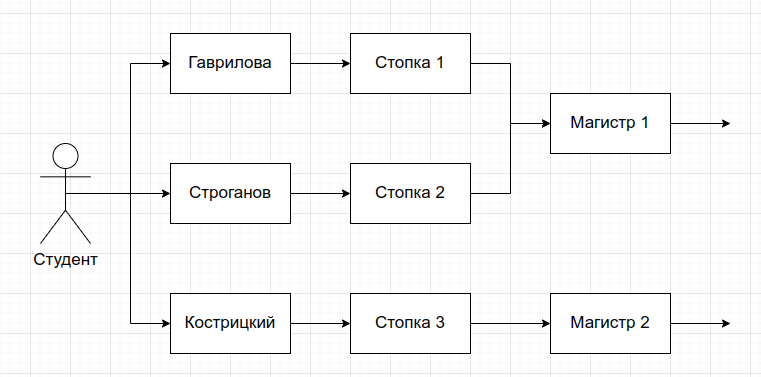
\includegraphics[width=\linewidth]{inc/flow.png}
	\end{center}
	\caption{Структурная схема потока}
\end{figure}
\FloatBarrier

\subsection*{Экзогенные и эндогенные переменные}
Эндогенные переменные этой модели -- время обработки задания $i$-м преподавателем и время решения бюрократических проблем $j$-м магистром.

Экзогенные переменные -- число студентов, сдавших комиссию и число студентов, получивших отказ.


\FloatBarrier
\begin{figure}[h]
	\begin{center}
		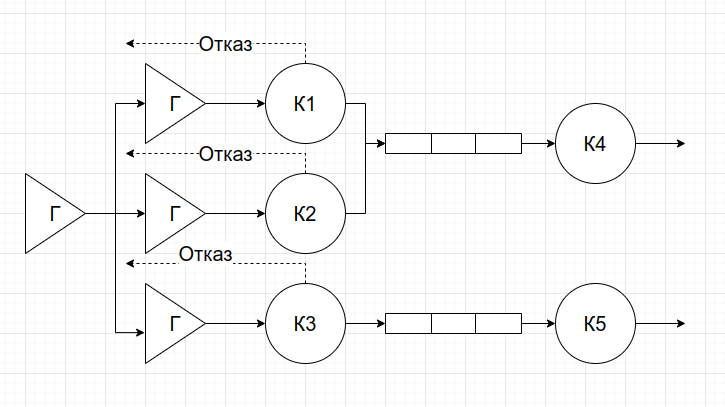
\includegraphics[width=\linewidth]{inc/flow1.png}
	\end{center}
	\caption{Модель}
\end{figure}
\FloatBarrier

\newpage

\subsection*{Равномерное распределение}
\textbf{Равномерное распределение} -- распределение случайной величины, принимающей значения, принадлежащие некоторому промежутку конечной длины, характеризующееся тем, что плотность вероятности на этом промежутке постоянна.


\subsubsection*{Вывод основных формул}
Пусть $A$ и $B$ -- границы промежутка равномерного распределения. Исходя из определения, плотность можно посчитать по формуле \ref{dens}:
\begin{equation}
	\label{dens}
	f(x)= 
	\begin{cases}
		C,& \text{если } x \in [A, B]\\
		0,              & \text{иначе}
	\end{cases}
\end{equation}

Одно из важнейших свойств плотности распределения -- нормированность. Его математическое представление выражено формуле \ref{prop}:
\begin{equation}
	\label{prop}
	\int_{-\infty}^{\infty} f(x) \,dx \ = 1
\end{equation}

Для равномерного распределения вычислим интеграл, учитывая свойства интеграла и формулу \ref{dens}:
\begin{equation}
	\label{viv}
	\int_{-\infty}^{\infty} f(x) \,dx \ = \int_{-\infty}^{A} 0 \,dx \ + \int_{A}^{B} C \,dx \ + \int_{B}^{\infty} 0 \,dx \ = \int_{A}^{B} C \,dx \ = C*(B - A)
\end{equation}

Вычислим плотность распределения, сравняв полученное в формулах \ref{prop} и \ref{viv}:
\begin{equation}
	\label{vivProb}
	C*(B - A) = 1 \rightarrow C = 1 / (B - A)
\end{equation}

Окончательная формула плотности распределения для равномерной случайной величины представлена на формуле \ref{dens1}:
\begin{equation}
	\label{dens1}
	f(x)= 
	\begin{cases}
		1 / (B - A),& \text{если } x \in [A, B]\\
		0,              & \text{иначе}
	\end{cases}
\end{equation}

Функцию распределения, зная плотность, можно рассчитать по формуле \ref{func}:
\begin{equation}
	\label{func}
	F_X(x) = \int_{-\infty}^{x} f_X(t) \,dt \ = 1
\end{equation}

Для равномерного распределения требуется рассмотреть три случая: $x < A$; $x \in [A, B]$; $x > B$. Рассчитывая интеграл для каждого из трёх случаев, получим формулу \ref{funcRes}:
\begin{equation}
	\label{funcRes}
	F_X(x)= 
	\begin{cases}
		0 & \text{если } x < A\\
		\frac{x - A}{B - A},& \text{если } x \in [A, B]\\
		1,              & x > B
	\end{cases}
\end{equation}

\newpage


\anonsection{Реализация}
В этом разделе будет приведены листинги кода реализации алгоритмов, продемонстрирована работа программы и построены таблицы с результатами.

\subsection*{Листинги кода}
Для реализации ПО был использован язык Python, так как имеется опыт разработки на нём.

На листинге 1 представлена реализация оператора.

На листинге 2 представлена реализация компьютера.

На листинге 3 представлена инициализация эндогенных переменных и подсчёт экзогенных параметров. 


\begin{lstinputlisting}[language=Python, caption=Реализация преподавателя, linerange={24-36}, 
	basicstyle=\footnotesize\ttfamily, frame=single,breaklines=true]{../src/operators.py}
\end{lstinputlisting}
\FloatBarrier


\FloatBarrier
\begin{lstinputlisting}[language=Python, caption=Реализация магистра, linerange={14-22}, 
	basicstyle=\footnotesize\ttfamily, frame=single, breaklines=true]{../src/processors.py}
\end{lstinputlisting}
\FloatBarrier

\FloatBarrier
\begin{lstinputlisting}[language=Python, caption=Инициализация эндогенных переменных и подсчёт экзогенных параметров, linerange={5-17}, basicstyle=\footnotesize\ttfamily, frame=single, breaklines=true]{../src/main.py}
\end{lstinputlisting}
\FloatBarrier


\subsection*{Полученные результаты}
Тестирование проводилось при различных параметрах числа обработанных заявок. 
Результаты приведены в таблице 1.

\FloatBarrier
\begin{table}[h]
	\caption{Таблица полученных значений}
	\centering
	\begin{tabular}{ | l | l | l | l |}
		\hline
		N студентов & N не принятых & N сдавших & Доля не принятых \\ 
		\hline
		100 & 8 & 92 & 0.08  \\
		\hline
		200 & 15 & 185 & 0.075  \\
		\hline
		500 & 35 & 465 & 0.07  \\
		\hline
	\end{tabular}
\end{table}

По результатам тестирования получилось, что средний процент отказов составляет $7,5$ процентов.